% =====================================================================
% 1. Problem and data (PRDL, Maria Martinez)
% Own block in depth: data loading, labels and split (T5; DECISIONS D1-D3,
% D12; block note 01). EDA (Oriana, T6) summarised and attributed.
% =====================================================================
\section{Problem and data}\label{sec:data}

\subsection{Task and dataset}

PTB-XL is a public collection of clinical 12-lead electrocardiograms of 10\,s, annotated by
cardiologists \cite{wagner2020ptbxl,ptbxl_physionet,pollard2026physionet}. Version 1.0.3 has \edaNRecordsAll{} records from
\edaNPatientsAll{} patients, at 500\,Hz and in a version downsampled to 100\,Hz; we use 100\,Hz, which
gives 1000 samples per lead, the sampling rate of the benchmark on this dataset
\cite{strodthoff2021deep}. Its licence (CC BY 4.0) was checked on the PhysioNet page. The task is
multi-label classification of the five diagnostic superclasses: normal ECG (NORM), myocardial
infarction (MI), ST/T change (STTC), conduction disturbance (CD) and hypertrophy (HYP). A record can
carry several superclasses, so a model outputs five logits, one per class, trained with a binary
cross-entropy each (Section~\ref{sec:evaluation}). The dataset fits the guidelines well: it is real and
curated, it has official folds and a published benchmark, and small models train on it with a laptop
GPU \cite{course_message_2011}.

\subsection{From the raw files to labelled tensors (my block)}

I wrote and checked the data pipeline (task T5, reviewed by Oriana). It turns the raw files into a
single cache and three data loaders, and each step was a decision with a reason.

\paragraph{Integrity.} Every file we use is hashed with SHA-256 and compared with the checksum list
published with the dataset, so a corrupted or modified file stops the pipeline instead of silently
changing the results.

\paragraph{Labels.} Each record lists diagnostic statements (SCP codes), each with a likelihood value.
A record gets superclass $c$ if any of its codes is a diagnostic statement of class $c$, whatever its
likelihood. The alternative of keeping only statements with a likelihood above zero was first proposed
by the AI assistant as ``the benchmark's rule'', without a source (Appendix~\ref{app:ai}). We checked it
against the example script distributed with the dataset, which ignores the likelihood, and against the
class counts of the PhysioNet page: only the rule we adopted reproduces them, and a test now checks the
counts on every run of the pipeline. The class shares are NORM \edaPrevAllNORMPct{}, MI
\edaPrevAllMIPct{}, STTC \edaPrevAllSTTCPct{}, CD \edaPrevAllCDPct{} and HYP \edaPrevAllHYPPct{} of the
labelled records, and \edaFracMultilabelAllPct{} of them carry more than one superclass.

\paragraph{Records without a superclass.} \edaNNosuperAll{} records have no diagnostic statement.
The exploratory analysis showed that almost all of them carry a rhythm statement and
\edaNNosuperRhythmOnly{} carry only rhythm statements, which in PTB-XL give no superclass. A target of
five zeros would tell the model ``none of these pathologies'', which is a false label, not a real
negative. They are therefore left out of training, validation and test (decision D12), and they are
spread evenly over the ten folds, so leaving them out does not unbalance any split. The benchmark does
the same: it selects ``only samples with at least one label in the given label selection''
\cite{strodthoff2021deep}. They were not wasted: the self-supervised pre-training of
Section~\ref{sec:strategies} needs no labels and used the training-fold ones.

\paragraph{Split.} We use the ten stratified folds shipped with the dataset, which keep all records of a
patient in the same fold: training folds 1--8, validation fold 9, test fold 10, as in the benchmark,
which trains ``on the first eight folds using the ninth and tenth fold as validation and test sets''
\cite{strodthoff2021deep}. Patient-wise folds matter because \edaNPatientsSeveralRecords{} patients have
more than one record; with a random split, records of the same patient could fall in training and test,
and the test score would partly measure memorisation of the patient. Folds 9 and 10 also have the best
labels: the dataset authors describe them as ``folds with a particularly high label quality that are
supposed to be used as validation and test sets'' \cite{wagner2020ptbxl}, and when they assigned ECGs of
a patient without the ``clean'' flag, they excluded the ninth and tenth fold \cite{wagner2020ptbxl}. In
our data, \edaFracValidatedByHumanTestPct{} of the test records are human-validated, against
\edaFracValidatedByHumanTrainPct{} of the training records. After removing the records without a
superclass, the splits have \edaNLabelledTrain{}, \edaNLabelledVal{} and \edaNLabelledTest{} records.

\paragraph{Normalisation.} Each lead is standardised (z-score) with the mean and standard deviation of
that lead over the training records only; validation and test reuse those values. Computing them on all
records would leak information about the evaluation folds into training. Two alternatives were
rejected: one global mean and deviation, because the leads have different amplitude ranges, and a
standardisation of each record by itself, because it removes the absolute amplitude of the record,
which we did not want to discard, since amplitude may carry diagnostic information (our reasoning, not a
tested or cited result).

% Shared float (common/make_floats.py). Figure: figures/eda_fold_distribution.pdf
\begin{figure}[htbp]
\centering
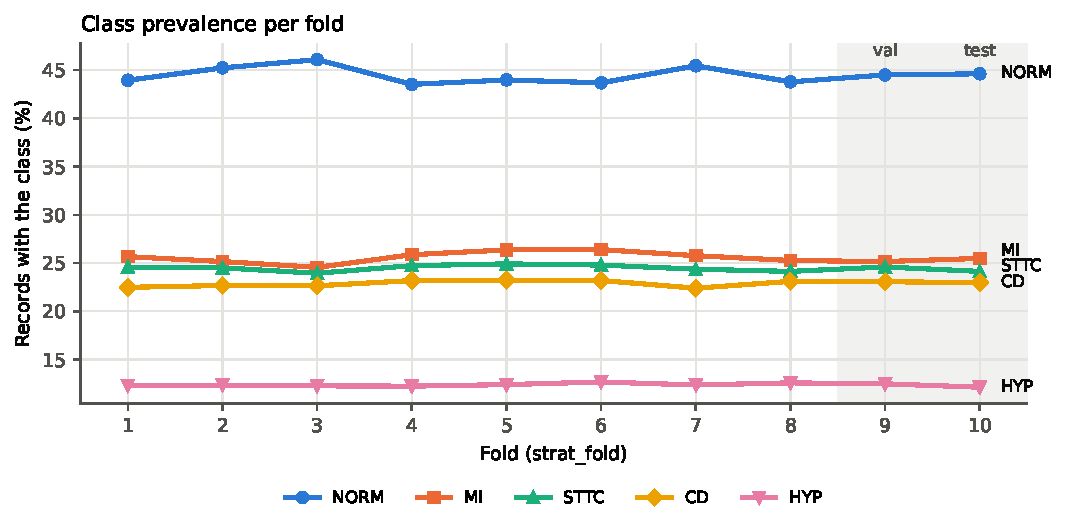
\includegraphics[width=\textwidth,height=0.42\textheight,keepaspectratio]{figures/eda_fold_distribution.pdf}
\caption[Class prevalence per fold]{Prevalence of each superclass in each of the ten official folds; the shaded folds are validation (9) and test (10).}
\label{fig:eda_fold_distribution}
\end{figure}


\subsection{Exploratory analysis (Oriana's block, summarised)}

The exploratory analysis was done by Oriana and reviewed by me. Three of its findings shaped the rest of
the project. The classes are imbalanced (Figure~\ref{fig:eda_class_counts}): HYP is the rarest, which is
why we report the AUROC of each class and choose F1 thresholds per class instead of a fixed 0.5. The
labels overlap (\edaFracMultilabelAllPct{} of the records have more than one), so the task is truly
multi-label. And the class shares are almost the same in the three splits
(Figure~\ref{fig:eda_fold_distribution}), so validation and test are representative of training. The
analysis also flagged \edaFracAnyQualityFlagAllPct{} of the records with a signal-quality note (baseline
drift, noise, extra beats); none was removed, so that the official folds stay intact.

% Shared float (common/make_floats.py). Figure: figures/eda_class_counts.pdf
\begin{figure}[htbp]
\centering
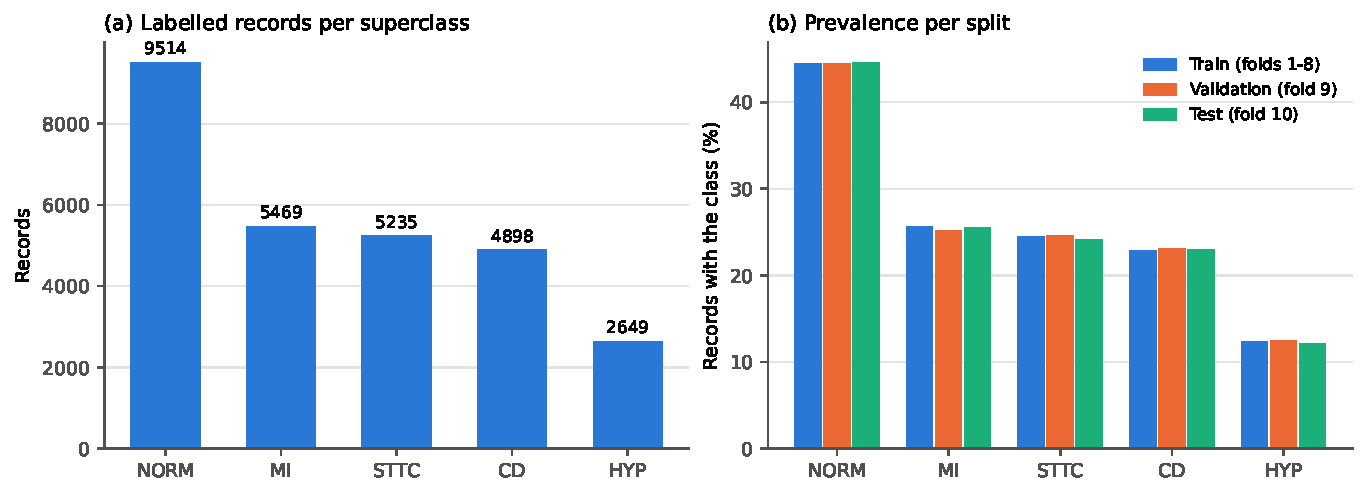
\includegraphics[width=\textwidth,height=0.42\textheight,keepaspectratio]{figures/eda_class_counts.pdf}
\caption[Records and prevalence per superclass and split]{PTB-XL superclasses. (a) Labelled records per superclass (a record may carry several). (b) Prevalence of each class in the training (folds 1--8), validation (fold 9) and test (fold 10) splits.}
\label{fig:eda_class_counts}
\end{figure}

